\begin{figure}[t]
    \centering
    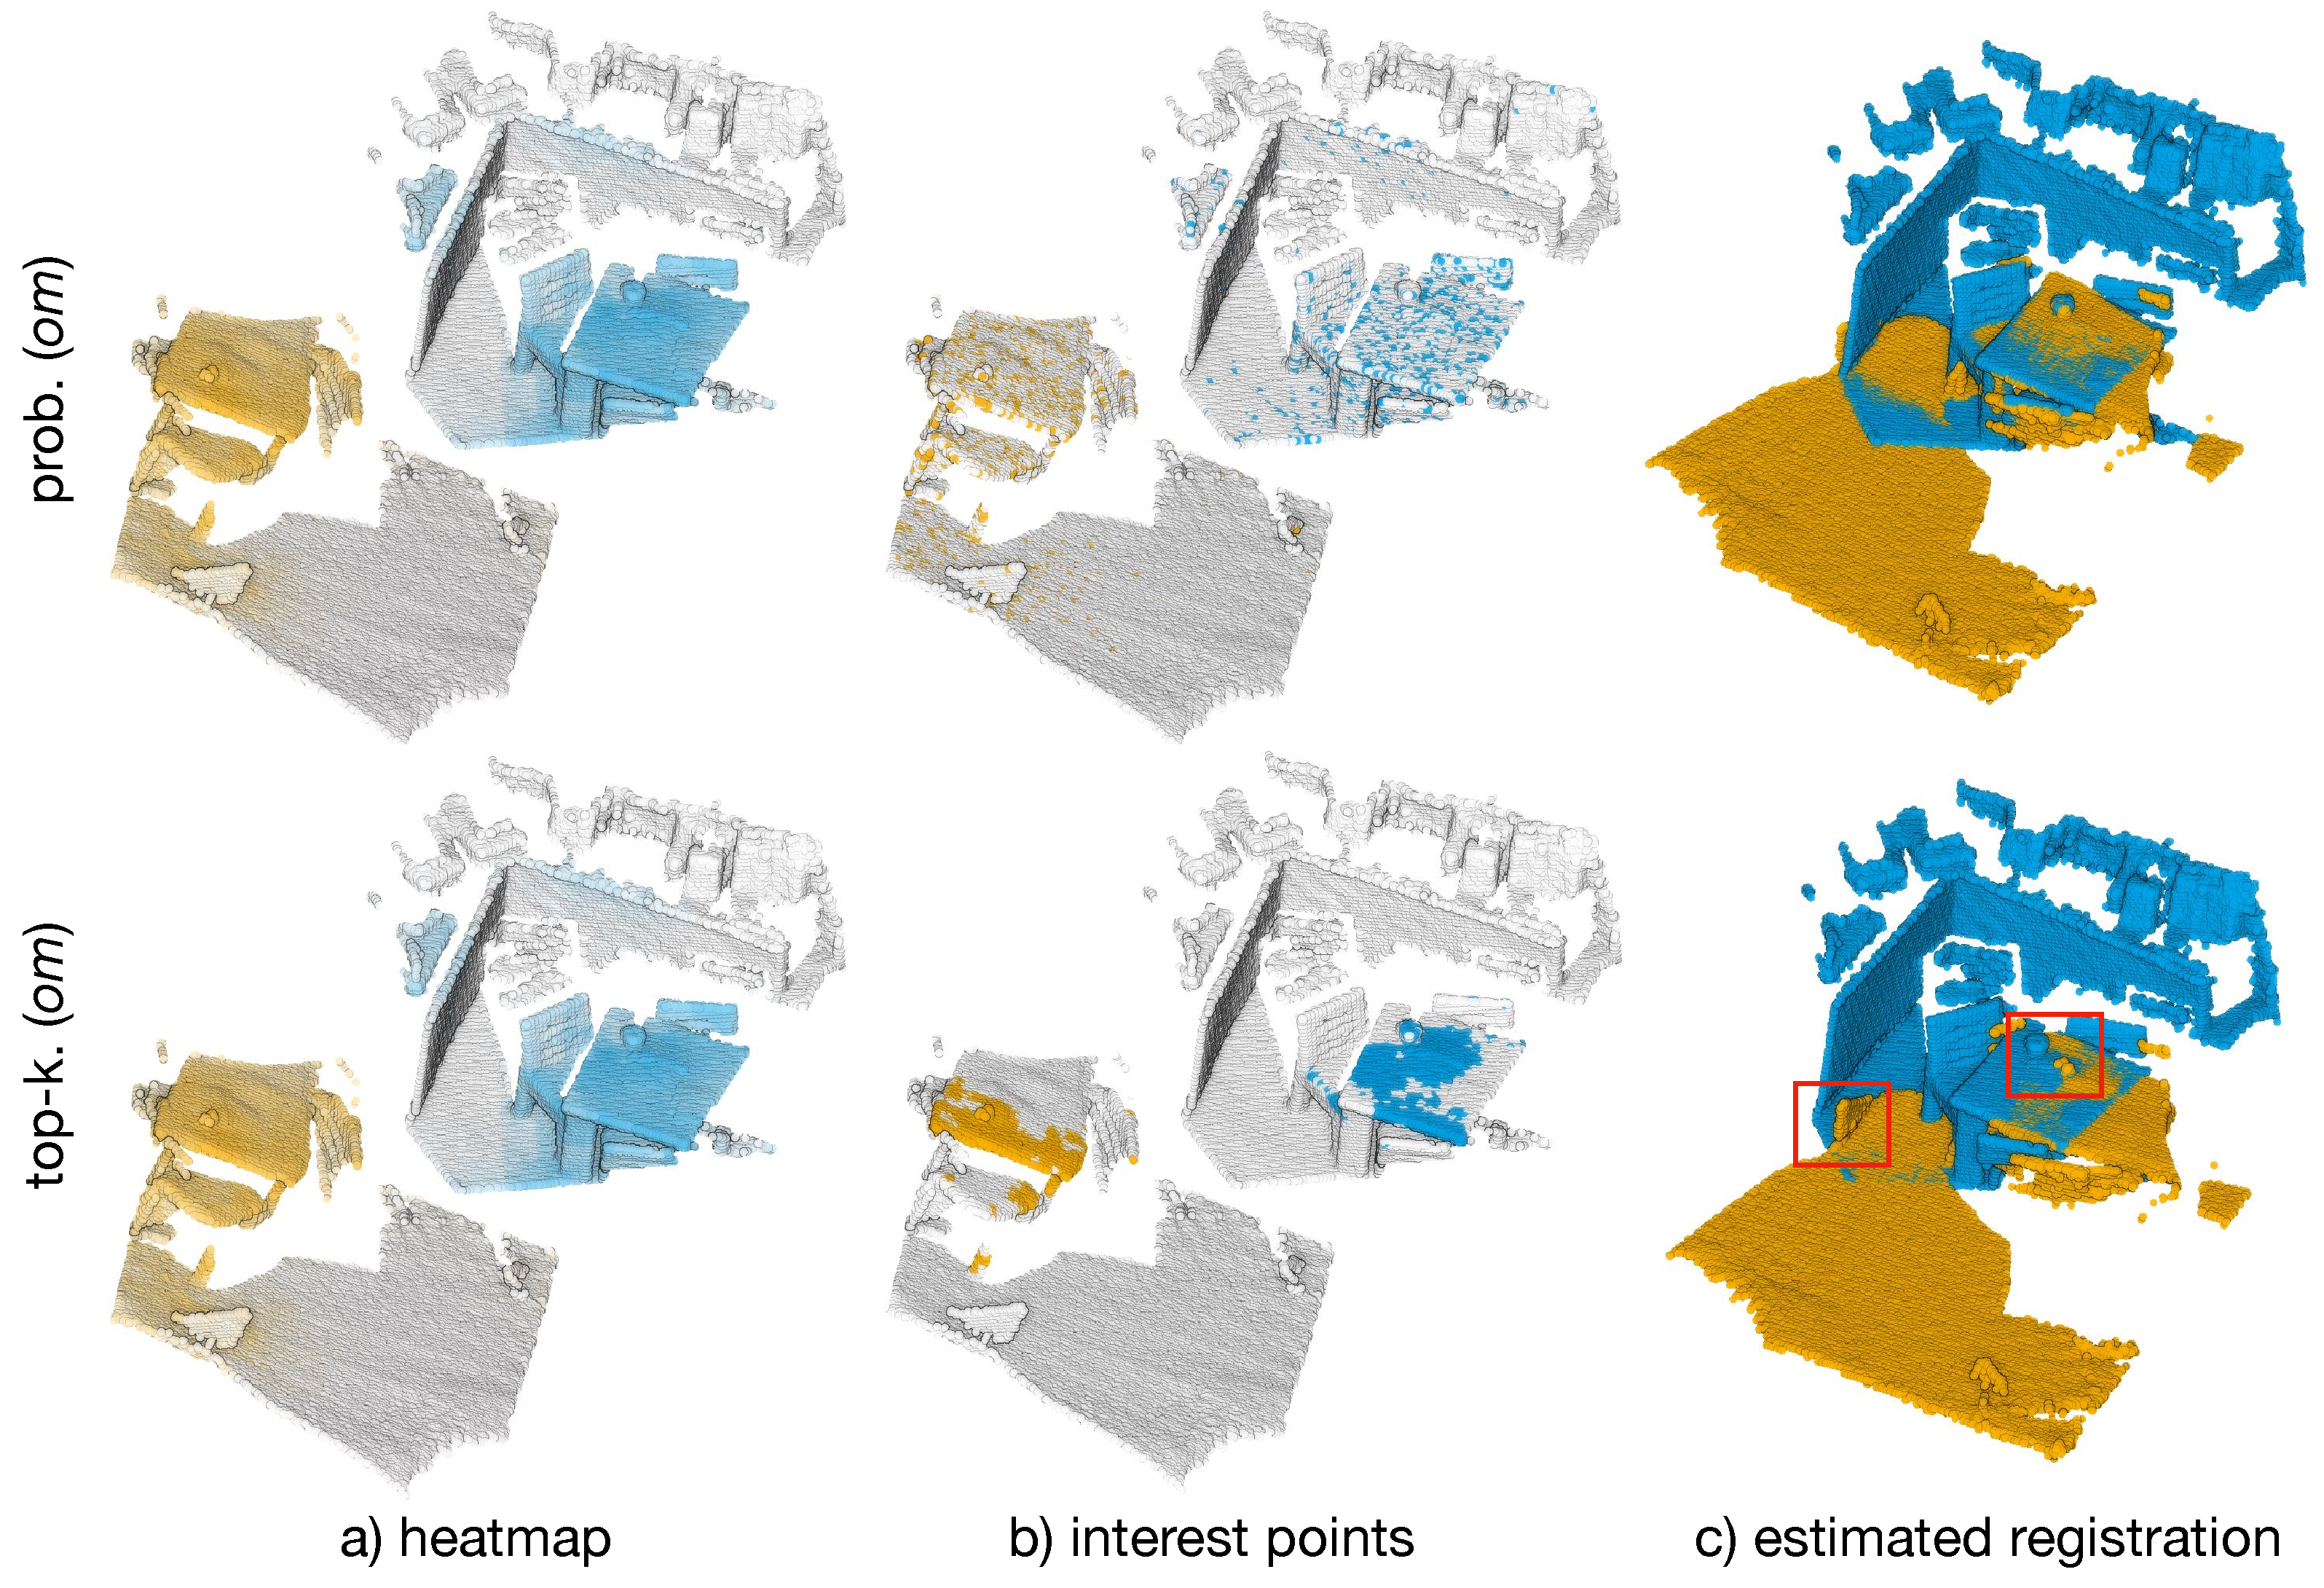
\includegraphics[width=\columnwidth]{figures/images/demo_sampling.pdf}
    \caption{\emph{Top-k ($om$)} sampling yields clustered interest points, whereas the points obtained with \emph{prob. ($om$)} sampling are more scattered and thus enable a more robust estimation of the transformation parameters.}
    \label{fig:sampling}
\end{figure}